\chapter{Statistical distance}


Suppose that we are given samples from two unkown distributions $P$ and $Q$, an 
important question to ask is: are $P$ and $Q$ equal?

\begin{figure}[H]
    \centering
    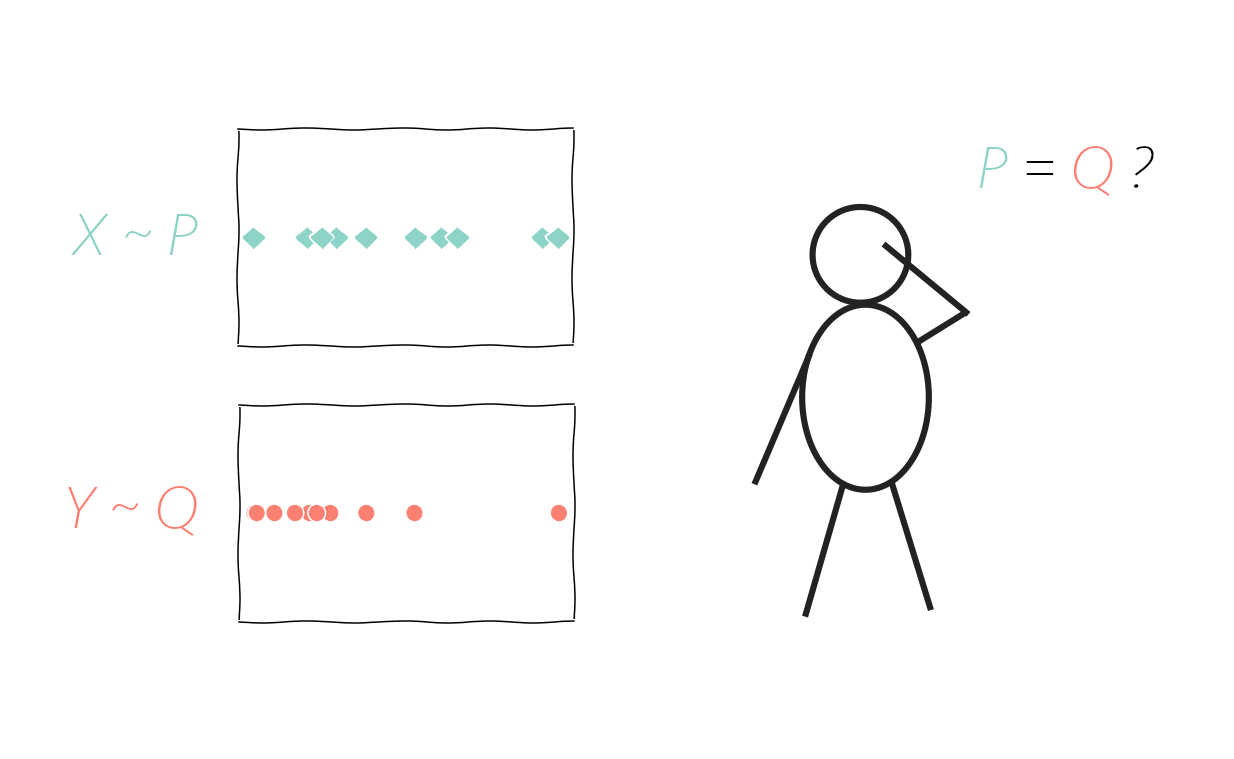
\includegraphics[width=.45\textwidth]{scatter_dist_question.png}
    % \caption{A comic}
    \label{fig:scatter_dist_questions} 
\end{figure}


The Integral Probability Metric (IPM) and f-divergence are two very rich and well studied
families of measures of "distance" between probability measures.

We start by introducing the Reproducing Kernel Hilbert Spaces (RKHS), which will serve as a 
building block for the maximum mean discrepancy, an important instance of IPM.

\section{Reproducing Kernel Hilbert Space}

We will begin by defining the kernel,

\subsection{Kernels}

\begin{definition}
    Let $\mathcal{X}$ be a non-empty set. A function 
    $k: \mathcal{X} \times \mathcal{X} \rightarrow \R$ is a kernel if 
    \begin{enumerate}
        \item $k$ is symmetric: $k(x, y) = k(y, x)$.
        \item $k$ is positive semi-definite, i.e. $\forall x_1, ..., x_n \in \mathcal{X}$,
        the "Gram Matrix" $K$, defined by $K_{ij} = k(x_i, x_j)$ is positive semi-definite
        \footnote{A matrix $M \in \R^{n\times n}$ is positive semi-definite if $\forall a \in \R^n$
        , $a^\intercal Ma \geq 0$}.
    \end{enumerate}
\end{definition}

It is easy construct new kernels since they are preserved under addition, multiplication and other operations. 
(See for example \cite{GrettonNotes}).

One example of a kernel -- and one of the most popular ones -- is the Gaussian Kernel defined on $\R^d$:

$$
    k(x, y) = \exp (-\gamma^{-2}\norm{x - y}^2)
$$

\subsection{Constructing the Reproducing Kernel Hilbert Space}

Let $\mathcal{X}$ be an arbitrary set and $\mathcal{H}$ a Hilbert space of real valued functions
on $\mathcal{X}$. As per general convention, addition and multiplication are define pointwise:

\begin{equation}
    \begin{array}{lll}
    (\lambda \cdot f)(x) & :=\lambda \cdot f(x) & \forall \lambda \in \R, \forall f \in \mathcal{H} \text { and } \forall x \in \mathcal{X} \\
    (f+g)(x) & :=f(x)+g(x) & \forall f \in \mathcal{H}, \forall g \in \mathcal{H} \text { and } \forall x \in \mathcal{X}
    \end{array}
\end{equation}

% One powerful fact about Hilbert spaces is that every Hilbert space admits an orthonormal basis, 
% and each vectorin the Hilbert space can be expanded as a series in terms of this orthonormal basis.

% For instance L2 blah blah

% $f \in L^1$ then we can decompose $f$ as follows:

% $$
%     f(x) = \int_{-\infty}^{\infty} \hat{f}(\omega) e^{2 \pi i x \omega} d \omega
%     = \inp*{\hat{f}}{\phi(x)}
% $$

We will now take a look at Hilbert spaces whose structure is highly linked with a kernel. 
Note that if we pick some $x \in \mathcal{X}$, then $k(x, .)$ is a function from $\mathcal{X}$ to $\R$.

\begin{definition}
    Let $\mathcal{H}$ be a Hilbert space of functions $f: \mathcal{X} \rightarrow \R$. 
    $\mathcal{H}$ is called a Reproducing Kernel Hilbert Space (RKHS) if there is a kernel k such that

    \begin{enumerate}
        \item $ k(x, .) \in \mathcal{H} \quad \forall x \in \mathcal{X}$
        \item $ \inp*{f}{k(x, .)} = f(x) \quad \forall f \in \mathcal{H}$
    \end{enumerate}

\end{definition}

Given the kernel $k$ it is convinient to define the feature map $\phi: \mathcal{X} \rightarrow \mathcal{H}$ as:

$$
    \phi(x) = k(x, .)
$$

The intuition is that in this space, we can view functions as linear combinations\footnote{
    Note that if $f(x)$ is an element of $\mathcal{H}$, then we write $f$ as the coefficients
    for the feature representation. 
} of features:

$$
    f(x) =  \inp*{f}{k(x, .)} = \inp*{f}{\phi(x)}
$$


The power of this setup -- which is known as the kernel trick -- is that inner products between
features (which can live in infinite spaces) are simple function evaluations; 
indeed by letting $f(x) = k(x, x\prime)$ we get

$$
    \inp*{k(x^\prime, .)}{k(x, .)} = k(x, x^\prime)
$$

Observe that both conditions imply that $k$ spans $\mathcal{H}$, i.e.

\begin{equation}
    \mathcal{H}=\overline{\operatorname{span}\{k(\cdot, x): x \in \mathcal{X}\}}
\end{equation}

Indeed is is possible to go the other way around\footnote{See the excellent lecture notes on 
RKHS \cite{BartlettNotes} for more details.} and first define the following vector space

\begin{equation}
    \operatorname{span}(\{\phi(x): x \in \mathcal{X}\})=\left\{f(\cdot)=
    \sum_{i=1}^{n} \alpha_{i} k\left(\cdot, x_{i}\right): n \in \N, x_{i} 
    \in \mathcal{X}, \alpha_{i} \in \R\right\}
\end{equation}

We can then equip this space with an inner product and to show that it is complete in order to create
a Hilbert Space (at which point we will have created a RKHS). 

\subsection{The kernel trick in action}

We will now show an application to illustrate both the power of the RHKS and to refine our intuition of it. 
Suppose that we have 
some data say $\{ x_i, y_i\}_{i \in [n]}$; we belive for example $y$ to be a smooth function of $x$ and we 
expect some independent aditive noise.

We can estimate $f$ as follows
\footnote{Note that it is not obvious how to implement the optimisation as $\mathcal{H}$ may be infinite. However,
this setup with a gaussian kernel is in fact equivalent to a Gaussian Processes, which can be easily
implemented in practice (see \cite{JordanNotes}).}
, pick an RHKS $\mathcal{H}$ with a gaussian kernes:

\begin{equation}
    f^{*}=\arg \min _{f \in \mathcal{H}}\left(
        \sum_{i=1}^{n} 
        \left(y_{i} - \inp*{f}{\phi\left(x_{i}\right)}_{\mathcal{H}} \right)^{2}
        + \Omega \norm{f}_{\mathcal{H}}^{2}\right)
\end{equation}

An amazing result is that an optimisation of the above form will always admit a representation of the
form:

\[
    f^{*} = \sum_{i=1}^{n} \alpha_{i} \phi\left(x_{i}\right)
\]
where $\alpha_{i} \in \mathbb{R}$ for all $1 \leq i \leq n$

This is known as the Representer Theorem (\cite{scholkopf2001generalized}); all it requires is that we be in the usual RHKS setup, and that
the regularisation be a strictly increasing\footnote{In our case regularisation is linear,
we thus simply need to pick $\Omega \geq 0$.} real valued function.
If we wish to approximate a prediction for some new sample $x$, we can do so as follows:


$$
    f^{*}(x) = \inp*{f^{*}}{\phi\left(x\right)} = 
    \sum_{i=1}^{n} \alpha_{i} \inp*{\phi\left(x_i\right)}{\phi\left(x\right)} =
    \sum_{i=1}^{n} \alpha_{i} k\left(x_i, x\right)
$$

It is precisely because the solution is of this form, that we may exploit the kernel trick. We can
also quickly see what the role of the kernel is. If for example, $k$ is the Gaussian Kernel, then
the solution will be a linear combination of scaled gaussians centered at the data points
\footnote{In fact this will always be the case when we can write $k\left(x_i, x\right) = \tilde{k}\left(x_i - x\right)$}. 

As a final remark we will explain the role of the penalty $\Omega \norm{f}_{\mathcal{H}}^{2}$; from 
statistical models, we now that this kind of term is known as regularisation and is supposed to help 
choose a "simpler" model. As we will now show, this is also the case here.

To see this, we will use Mercer's Theorem -- a Generalisation of the spectral theorem for positive-semidefinite
matrices\footnote{Recall that our Kernel $k$ is a generalisation of a positive-semidefinite Matrix}.

\begin{theorem}[Mercer's] 

Suppose $k$ is a continuous positive semi-definite kernel on a compact set $\mathcal{X}$, then if
, $\forall f \in L_{2}(\mathcal{X})$

\[
\int_{\mathcal{X}} k(u, v) f(u) f(v) d u d v \geq 0
\]

then $k$ has the following decomposition

\begin{equation}
    k(u, v)=\sum_{i=1}^{\infty} \lambda_{i} \psi_{i}(u) \psi_{i}(v)
\end{equation}

Where $\{\psi_i\}$ forms an orthonormal basis of $L_2(\mathcal{X})$, 
such that the corresponding sequence of eigenvalues $\{\lambda_i\}$ are non-negative.

Where the convergence is absolute and uniform, that is,
\[
\lim _{n \rightarrow \infty} \sup _{u, v}\left|k(u, v)-\sum_{i=1}^{n} \lambda_{i} \psi_{i}(u) \psi_{i}(v)\right|=0
\]
    
\end{theorem}

We can now use this decomposition of the Kernel to get further insight, using Mercer's theorem we can 
thus write -- assuming the conditions are met:

$$
    k \left(x, x^{\prime}\right)=\sum_{i=1}^{\infty} 
    \underbrace{\left[\sqrt{\lambda_{i}} \psi_{i}(x)\right]}_{\phi_{i}(x)} 
    \underbrace{\left[\sqrt{\lambda_{i}} \psi_{i}\left(x^{\prime}\right)\right]}_{\phi_{i}\left(x^{\prime}\right)}
$$

We can thus rewrite the solution as follows

$$
    f^{*}(x) = \sum_{i=1}^{n} \alpha_{i} k\left(x_i, x\right) = 
    \sum_{i=1}^{\infty} \phi_i\left(x\right) 
    \sum_{j=1}^{n} \alpha_{j}  \phi_i\left(x_j\right) = 
    \sum_{i=1}^{\infty} \sqrt{\lambda_{i}} \psi_{i}(x) f^{*}_i 
$$

Note that due to the $\Omega \norm{f}_{\mathcal{H}}^{2}$ penalty, $f^{*}_i$ must decay for higher values of $i$. Note that
for example in the Fourier Transform
, in the basis $\{\psi_i\}$, higher values of $i$ correspond to higher 
frequency functions; similarly, for the Gaussian Kernel, higher indicies basis functions correspond to 
higher frequecies\footnote{In the fourier space, we have the following
basis $\psi_\omega = \exp (2\pi i x \omega)$}. Thus, a higher $\Omega$ will force a faster decay on $f_i$ and thus result in smoother functions
-- in principle, this will reduce overfitting. 

\begin{figure}[H]
    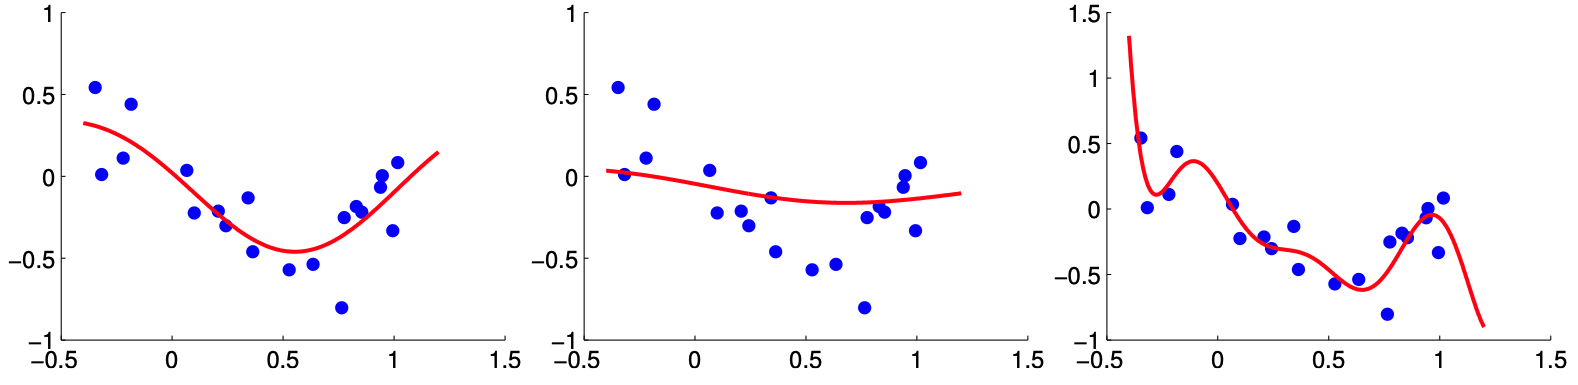
\includegraphics[width=1\textwidth]{kernel_smoothness.jpg}
    \caption{Small RKHS norm results in smooth functions. 
    From left to right $\Omega = .1$, $\Omega = 10$, $\gamma = 1\mathrm{e}{-7}$, 
    we fix the Gaussian kernel with $\gamma = 0.6$}
    \label{fig:kernel_smoothness} 
\end{figure}




\section{Integral Probability Metric}

\subsection{Introduction}

We now turn to the question of statistical distance, i.e. given samples of $P$ and
$Q$, how can we determine if $P = Q$?

Observe that if two random variables $X$, $Y$ share the same distribution, then 

$$
\E(g(X)) = \E(g(Y))
$$

for any continuous and bounded function $g : \R \rightarrow \R$. 
It turns out that the reciprocal statement holds. (See \cite{TwoSampleTestGrettonBernhard})

This motivates the following construction

$$
D_\mathcal{F} (P, Q) = 
\sup _{g \in \mathcal{F}} \mid \mathop{\E}_{X \sim P} g(X) - \mathop{\E}_{Y \sim Q} g(Y) \mid
$$

where $\mathcal{F}$ is a class of real-valued bounded measurable functions.

% See for example \cite{sriperumbudur2009integral} for a detailed analaysis

This defines a rich class of distance measures known as 
integral probability metrics (IPMs) (see \cite{muller1997integral}). Depending
on how we choose $\mathcal{F}$ we may end up with different popular distance measures, such as
the Wasserstein distance or the Total variation distance to name a few. 

The goal is to craft an $\mathcal{F}$ that is "expressive" enough so that the IPM vanishes iff $P = Q$,
and on the other hand, we need $\mathcal{F}$ to be "restrictive" enough so as to have fast and 
reliable guarantees of the empirical estimate of the IPM (\cite{TwoSampleTestGrettonBernhard}.)


\subsection{MMD}

Consider $\mathcal{F}=\left\{f:\|f\|_{\mathcal{H}} \leq 1\right\}$, this is known
as the maximum mean discrepancy (MMD). Where $\mathcal{H}$, is a reproducing kernel Hilbert space 
(RHKS) with $k$ as its reproducing kernel. 

We will next extend the notion of the feature map to the \textbf{embedding of probability distributions}. 
Recall that if $\phi$ is the associated feature map to the kernel $k$ from 
RKHS $\mathcal{H}$ then we have $g(x) = \inp*{g}{\phi(x)}$.

We define $\mu_P \in \mathcal{H}$, s.t. $\forall g \in \mathcal{H}$, we have that
$\mathop{\E}_{X} g(X) = \inp*{g}{\mu_P}$. We will now show under which conditions $\mu_P$ exits.

\begin{lemma}\label{embedding_existance}
    If k is measurable and $\mathop{\E}_{X} \sqrt{k(X, X)} < \infty$ then
    $\mu_P \in \mathcal{H}$
\end{lemma}

\begin{proof}
\begin{align*}
    \left|\E_{X} g(X)\right| &\leq 
    \E_{X}|g(X)| \\
    &=
    \E_{X}\left| \inp*{g}{\phi(X)}_{\mathcal{H}}\right| \\
    &\leq
    \E_{X} \norm{g}_{\mathcal{H}} \norm{\phi(X)}_{\mathcal{H}} \\
    &= \norm{g}_{\mathcal{H}} \E_{X} \sqrt{k(X, X)}
\end{align*}
Thus $E_{X} g(X)$ is a bounded linear operator $\forall g \in \mathcal{F}$, and by the
Riesz representer theorem it follows that there exists a $\mu_P \in \mathcal{H}$
s.t. $\mathop{\E}_{X} g(X) = \inp*{g}{\mu_P}$. 
\end{proof}


We can also see that the mean embedding of the distribution $P$ is the expectation under $P$
of the feature map $\phi$.

$$
    \mathop{\E}_{X \sim P} g(X) = 
     \inp*{g}{ \mathop{\E}_{X \sim P} \phi(X)} = \inp*{g}{\mu_P}
$$

Asumming Lemma \ref{embedding_existance} -- and using Cauchy-Schwartz, 
we can explicitly solve the MMD in terms of the mean embeddings:

\begin{align*} 
    \text{MMD}_\mathcal{F} (P, Q) 
    &= 
    \sup _{g \in \mathcal{F}} \mid \mathop{\E}_{X \sim P} g(X) - \mathop{\E}_{Y \sim Q} g(Y) \mid \\
    &= 
    \sup _{g \in \mathcal{F}} \mid \inp*{g}{\mu_P - \mu_Q} \mid \\
    &=
    \norm{\mu_P - \mu_Q}_\mathcal{H}
\end{align*}

We can therefore see the MMD as the feature mean difference of the distributions; we can further
expand this expression to get the result as a function of the kernel.

\begin{align*}
    \text{MMD}_\mathcal{F}^2 (P, Q)
    &=
    \norm{\mathop{\E}_{X \sim P} \phi(X)  - \mathop{\E}_{Y \sim Q} \phi(Y) }_\mathcal{H}^2 \\
    &= \mathop{\E}_{X \sim P} \mathop{\E}_{X^\prime \sim P} \inp*{\phi(X)}{\phi(X^\prime)} - 
    2 \mathop{\E}_{X \sim P} \mathop{\E}_{Y \sim Q} \inp*{\phi(X)}{\phi(Y)} +
    \mathop{\E}_{Y \sim Q} \mathop{\E}_{Y^\prime \sim Q} \inp*{\phi(Y)}{\phi(Y^\prime)} \\
    &= \mathop{\E}_{X \sim P} \mathop{\E}_{X^\prime \sim P} k \left( X, X^\prime \right) - 
    2 \mathop{\E}_{X \sim P} \mathop{\E}_{Y \sim Q} k \left( X, Y \right) +
    \mathop{\E}_{Y \sim Q} \mathop{\E}_{Y^\prime \sim Q} k \left( Y, Y^\prime \right)
\end{align*}

Note that we can straightforwardly estimate with samples the above expression; all the we require is 
to specify a kernel: \textit{so how do we choose a kernel}?

We need to ensure that $\text{MMD}(P, Q) = 0$ iff $P = Q$, in other words, $\mu_P$ needs to be injective
as a function of $P$. Intuitively this means that $\mathcal{F}$ needs to be expressive enough to 
reproduce enough continuous functions. One can show that to check if the resulting embedding 
$\mu_P$ is injective, we may check either of these sufficient conditions (\cite{sriperumbudur2008injective}) 
on the Kernel $k$:

\begin{enumerate}
    \item $k$ is a universal kernel.
    \item $k$ is a convolution kernel on $\R^n$, for which the Radon-Nikodym derivative of 
    its inverse Fourier transform is supported almost everywhere.
\end{enumerate}

The first condition is basically what we knew intuitively: 
If we consider a compact metric space, say $(\mathcal{X}, d)$, then a Kernel $k$ on $\mathcal{X}$
is called universe if the corresponding RKHS is dense 
in the space $C(\mathcal{X})$ of all continuous functions. The drawback is that the input space $\mathcal{X}$ needs to be compact -- which excludes $\R^n$; 
this means that we cannot use universality to check our gaussian kernel. Luckly the second condition
is enough.

Assuming $k$ is a bounded continuous positive definite function, then if we can write
$k(x, y) = \psi (x - y)$ we say that $k$ is a convolution kernel.

From inspection it is clear that the gussian kernel is convolutional

$$
    k(x, y) = \exp (-\gamma^{-2}\norm{x - y}^2)
$$

Recall that the fixed point of convolution is the gaussian, which trivially implies
that the inverse Fourier transform of a gaussian is supported everywhere. 
 This means that the gaussian kernel satisfies the second
condition, and it therefore generates an injective embedding $\mu_P$.

We note that HSIC is to MMD, what the Mutual Information is to the Kullback–Leibler divergence.

\subsection{The case for MMD}

In their study, \cite{sriperumbudur2009integral}) argue that the "IPM is much
simpler than estimating f-divergences, and that the estimators
are strongly consistent while exhibiting good rates of conver-
gence. IPMs also account for the properties of
the underlying space M through the Kernel in case of MMD. This is especially
useful when considering disjoint supports between P and Q"

Another argument for the MMD, is that we only need to choose a kernel; in contrast, 
when applying the f-divergence in practie we need to quantize in order to get an 
emprical distribution. While both can be seen as a hyperparameter, the effect of 
discretisation is not as obvious as that of choosing a kernel. 

\section{f-divergence}

Generalisation of the usual divergence, exploit jensen.

Talk about f-divergence, and give proof that D(p, q) >=0 and eq iff p == q

Talk about IPM vs $f-$divergence. 

To test whether two random variables are independent $X, Y$

talk about L1 being f-divergence


\section{Large deviations}

Consider making this into a chapter

\subsection{Hoeffding}

\subsection{Sanov}

\subsection{K-means}





